\chapter{Introducción}\label{cap.introduccion}
Este Trabajo Fin de Grado (TFG) se encuadra en un entorno educativo para enseñar a programar robots. En este primer capítulo se expondrá tanto el contexto en el cual se sitúa este proyecto como la motivación principal que ha llevado a su desarrollo. Cabe comenzar por realizar una explicación general de qué es la robótica y de las aplicaciones crecientes que está ofreciendo a la sociedad. 

Gran parte de la funcionalidad de los robots reside en su software. Intervienen en este aspecto diferentes elementos como los simuladores, las bibliotecas de código y los middlewares de robótica, los cuales se comentarán en la segunda sección del capítulo. En la tercera sección se describirá brevemente el panorama de la educación en robótica y el entorno docente JdeRobot-Academy en el que se ha desarrollado este TFG. La intención es extender precisamente este entorno docente con dos nuevos ejercicios que involucren algún problema de robótica. A la hora de desarrollar un sistema robótico hay numerosas cuestiones que abordar y solucionar,  la mayoría de las cuales el entorno docente soluciona y oculta al estudiante, que se puede centrar en los algoritmos robóticos más que en cuestiones auxiliares aunque necesarias.

\section{Robótica}
A lo largo de la historia, el hombre siempre se ha apoyado en la ciencia y la tecnología para facilitarle la vida, para lo cual ha ideado, construido y empleado herramientas o máquinas que consiguen reducir su carga de trabajo. La robótica es una rama de la ingeniería que emplea la informática para diseñar y desarrollar sistemas automáticos que permitan facilitar la vida del ser humano, e incluso sustituirle en determinadas tareas. Esta rama involucra conceptos de diversas disciplinas, tales como la física, las matemáticas, la electrónica, la mecánica, la inteligencia artificial, la ingeniería de control, etc. Mediante todas estas disciplinas unidas convenientemente se pueden diseñar máquinas que ejecuten distintos comportamientos autónomos en función de su propósito. Estas máquinas se denominan “Robots”.

El término “Robot” surge a partir de la palabra de origen checo \textit{robota}, cuyo significado es “trabajo forzado”. Fue el dramaturgo y autor checoslovaco Karel Capek, en su obra de teatro R.U.R (\textit{Robots Universales de Rossum}) en 1921, quien introdujo dicha palabra por primera vez en la historia. Aunque ese es el origen de la palabra, no lo fue así del concepto y del campo de estudio, ya que en aquel entonces era únicamente un término relacionado con la ciencia ficción. Desde el término de robot acuñado por Isaac Asimov en 1950, estos sistemas autónomos han experimentado un crecimiento exponencial en cuanto a su complejidad, versatilidad, autonomía y, sobre todo, presencia en multitud de ámbitos. Aquellos sistemas operados por seres humanos empiezan a disponer de un sistema de control propio programable, que les permite desempeñar aquellas tareas repetitivas o de riesgo para las personas, englobando actividades básicas y de difícil realización, hasta el punto en el que nos encontramos en la actualidad, en el cual existen múltiples ejemplos que integran la robótica en diferentes campos y tareas. Los robots comerciales e industriales son ampliamente utilizados y realizan tareas de forma más exacta o más barata que los humanos. Los robots también se emplean en trabajos demasiado sucios, peligrosos o tediosos para los humanos. En definitiva, un campo cada vez más popular y en expansión constante.

\begin{figure}[H]
  \begin{center}
    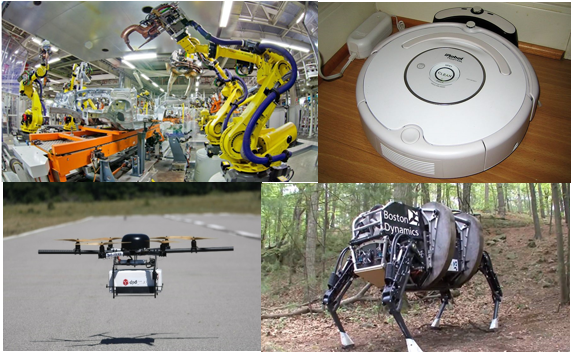
\includegraphics[width=0.8\textwidth]{figures/robots.png}
		\caption{Robots modernos}
		\label{fig.robots}
		\end{center}
\end{figure}

Hoy en día no solamente nos rodean los robots industriales, como los involucrados en cadenas de envasado de alimentos o cadenas de producción, sino que los robots cobran cada vez más importancia en entornos alternativos, como el doméstico entre otros, algunos de los cuales quedan representados en la \textbf{Figura 1.1}. Las aspiradoras robóticas (Roomba, Dyson, Xiaomi,…) han llegado a los hogares con éxito para realizar una tarea doméstica necesaria. Por otro lado, los vehículos de transporte aumentan cada vez más la tecnología robótica incorporada, como son los módulos de aparcamiento automático, u otros más avanzados como los asistentes de conducción autónoma (autopiloto de Tesla), o los recientes prototipos de coches autónomos que han lanzado grandes empresas como Google o Apple. Otros ámbitos, como el militar con máquinas capaces de desactivar bombas o realizar misiones de rescate, el de la medicina con el ejemplo del robot DaVinci que permite operar a un paciente desde cualquier parte del mundo con mayor precisión que la humana, o el de la logística en almacenes de Amazon tampoco están exentos de presencia robótica. Incluso se está trabajando para construir robots androides o humanoides capaces de desarrollar “comportamientos inteligentes” como el robot Asimo de Honda (\textbf{Figura 1.2}) o TOPIO, creado por TOSY Robotics (\textbf{Figura 1.3}), que puedan desempeñar tareas de interacción con herramientas y entornos humanos, ya sea con fines experimentales como el estudio de la locomoción bípeda, o incluso como auxiliar para la tercera edad o personas con movilidad reducida.

\begin{figure}[h]
	\centering
	\begin{minipage}[h]{.48\linewidth}
		\centering
		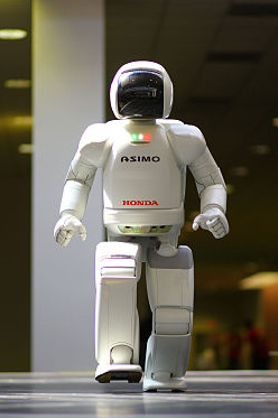
\includegraphics[width=.5\linewidth, height=7cm]{figures/asimo.png}
		\captionof{figure}{Robot Ásimo}
		\label{fig:asimo}
	\end{minipage}
	\begin{minipage}[h]{.48\linewidth}
		\centering
		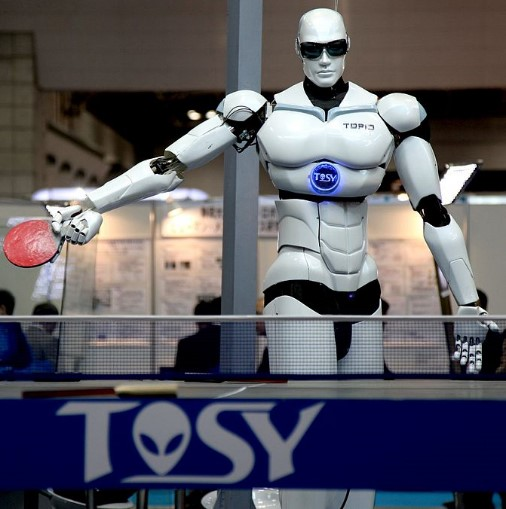
\includegraphics[width=.7\linewidth, height=7cm]{figures/topio.jpg}
		\captionof{figure}{Robot TOPIO}
		\label{fig:topio}
	\end{minipage}
\end{figure}

El abanico de aplicaciones que pueden involucrar sistemas robóticos es tan extenso como la imaginación de la comunidad dedicada a crearlos, por lo que tareas que nunca habíamos imaginado automatizadas son ahora labores totalmente robotizadas, como puede ser la agricultura de precisión a través de drones con análisis de imágenes térmicas y multiespectrales para aumentar el rendimiento de las explotaciones agrícolas, la automatización de aplicaciones anestésicas de bajo nivel e incluso competiciones deportivas de robots. 

Es difícil no parase a pensar en la potencia que tiene esta rama de la ciencia y la tecnología, y no sólo eso, sino también en la que puede alcanzar, ya que esto es solamente el principio. Con todo lo anterior, sale a relucir la utilidad de esta área de desarrollo, que permitirá en el futuro ganar en comodidad, economía e incluso salud. Es importante advertir la importancia de dominar esta disciplina en el futuro cercano, ya que será la llave que abrirá la puerta hacia un mundo más sencillo y seguro a través de la automatización.

\section{Software Robótico} 
Queda de manifiesto que para la totalidad de los ejemplos mencionados es necesario que el comportamiento del software que controla dichos robots debe ser robusto. Es por eso que se divide en distintas capas (\textit{drivers}, \textit{middleware} y aplicaciones), cuya arquitectura es distinta según sea su aplicación final.

Lejos ya de ser controlados por personas, la mayoría de los robots están dotados de una autonomía que les permite desempeñar la tarea o tareas para las cuales han sido diseñados sin la mediación de terceros. Que dispongan de esta característica es posible gracias al minucioso desarrollo de sistemas complejos que constan de un software tal que compone algo parecido a una inteligencia autónoma.
El desarrollo de software robótico parte de ciertos requisitos o tareas, entre las que se incluyen circuitos de retroalimentación, filtrado de datos, control, búsqueda de caminos y localización entre muchas otras. En los últimos años, han surgido numerosas plataformas de desarrollo de software para aplicaciones robóticas, también llamados \textit{middleware} robóticos. Los simuladores también son ingredientes habituales en el desarrollo de software robótico, permiten realizar las pruebas pertinentes, depurar los fallos programar una versión funcional del robot evitando el alto coste del proceso real una y otra vez. Estas herramientas son indispensables hoy en día para generar el conjunto de comandos codificados que indican al robot y a su sistema electrónico las acciones a realizar, así que entraremos un poco más en detalle en el siguiente apartado. Finalmente, las bibliotecas son de gran utilidad para generar el conjunto de comandos codificados que conforman el comportamiento del robot.

\subsection{Middlewares robóticos}
Los \textit{middleware} robóticos pueden definirse como entornos o \textit{frameworks} para el desarrollo de software para robots, es decir, software que conecta aplicaciones o componentes software para soportar aplicaciones complejas y distribuidas. Estos entornos suelen incluir \textit{dirvers} para controlar los sensores y los actuadores de los robots, arquitectura software para las aplicaciones que se van a crear, bloques de funcionalidad robótica ya resuelta y otra serie de herramientas como simuladores, visualizadores… Es por eso que hay muchas reseñas del \textit{middleware} en las que se hace referencia a él bajo el nombre de “pegamento para software”. El \textit{middleware} más extendido en el mundo es ROS…

	\textbf{Robot Operating System (ROS)\footnote{\url{http://www.ros.org/}}}
	
Es una plataforma de software libre para el desarrollo de software de robots que provee la funcionalidad de un sistema operativo en un clúster heterogéneo, como el control de dispositivos de bajo nivel, la abstracción del hardware, el control de dispositivos de bajo nivel y mecanismos de intercambio de mensajes entre procesos, todos ellos de vital importancia para el desarrollo en este campo. Una de las razones que hace que ROS sea el \textit{framework} más utilizado es que, aunque se diseñó para ser utilizado principalmente en sistemas UNIX, se ha adaptado de forma que pueda utilizarse también en los otros sistemas operativos principales como Fedora, Debian,  Windows, MacOS X, Arch, Slackware, Gentoo u OpenSUSE, llegando incluso a abrir la puerta a la construcción de aplicaciones multiplataforma.

Existen algunos otros interesantes como: 

	\textbf{Orocos}
	
También encaja en el grupo de las plataformas de software libre para control avanzado de máquinas y robots basado en C++.
 
	\textbf{Orca}
	
Un proyecto de software libre para aplicaciones de índole robótico que permite crear aplicaciones algo más complejas al estar orientado a componentes.

	\textbf{Urbi}
	
\textit{Middleware} multiplataforma de código abierto en C++ que, utilizada de forma conjunta con ROS, permite desarrollar aplicaciones para sistemas complejos y completos.

	\textbf{JdeRobot}
	
Plataforma para desarrollar aplicaciones robóticas y de visión artificial, que involucra nodos programados con varios lenguajes de programación y que es compatible con \textit{middlewares} de comunicaciones como ICE o ROS.

\vspace{1cm}
Una de las tareas de las que se encarga el \textit{middleware} es de conectar nuestro hardware, real o simulado, con nuestra aplicación en desarrollo.

\subsection{Simuladores robóticos}
Generalmente, el diseño y puesta en escena de un robot es costoso y caro, por lo que no es aconsejable correr el riesgo de que el código implementado contenga errores que salgan a la luz en el momento de probarlo, ya que esto puede generar malfuncionamientos e incluso rotura del hardware. Es por eso que el paso previo a llevar el código a la máquina consiste en probarlo antes en un simulador orientado a este tipo de aplicaciones, lo que permite un desarrollo seguro y económico. Algunos de los simuladores más usados son:

	\textbf{Gazebo}\footnote{\url{http://gazebosim.org/}}
	
Es el simulador 3D de código abierto más distribuido, bajo licencia Apache 2.0. Destaca sobre los demás por sus motores de físicas, motor de renderizado avanzado y soporte para \textit{plugins} de robots y sensores, además de un amplio repertorio de robots comerciales y sus correspondientes sensores y actuadores. Además, se integra bien con ROS, permitiendo usar exactamente el mismo código de la simulación en el robot real.

	\textbf{Stage}
	
Esta herramienta permite simular robots móviles en el plano bidimensional o en el tridimensional, integrable con ROS.

	\textbf{Webots}
	
Simulador de robótica avanzada que permite definir modelos propios y su física, escribir controladores para ellos y hacer simulaciones a gran velocidad. 

\subsection{Bibliotecas}
Queda claro que en el proceso de desarrollo de la parte software en robótica hay que resolver multitud de problemas clásicos y funcionalidades básicas además de las específicas para la aplicación en cuestión, ardua tarea para el programador que debe no sólo integrarlas en su proyecto, sino también abordarlas desde cero. Con el propósito de evitar esta situación, existen las llamadas bibliotecas, que no son más que conjuntos de implementaciones de código que ofrecen una interfaz bien definida para la funcionalidad que invocan. Su fin es ser utilizada por otros programas, independientes y de forma simultánea. Las bibliotecas pueden vincularse a un programa (o a otra biblioteca) en distintos puntos del desarrollo o la ejecución de dicho programa. Algunas de las bibliotecas utilizadas en robótica son: 
\begin{itemize}
	\item OpenCV \footnote{\url{https://opencv.org/}}: Es una biblioteca libre de visión artificial originalmente desarrollada por Intel. Contiene más de quinientas funciones que abarcan una gran gama de áreas en el proceso de visión, como reconocimiento de objetos, reconocimiento facial, calibración de cámaras, visión estéreo y visión robótica. Originalmente, OpenCV fue escrita en C++. Actualmente, la librería dispone de interfaces en C++, C, Python, Java y MATLAB. Es multiplataforma, existiendo versiones para GNU/Linux, Mac OSX, Windows y Android. 
 \item PCL \footnote{\url{http://pointclouds.org/}}: Se utiliza para el procesamiento digital de imágenes mediante el tratamiento de nubes de puntos aleatorios. Contiene numerosos algoritmos de última generación que incluyen filtrado, estimación de características, reconstrucción de superficies, ajuste de modelos y segmentación entre otros. Para simplificar el desarrollo, PCL se divide en una serie de bibliotecas de código más pequeñas, que se pueden compilar por separado. Es multiplataforma y ha sido compilado con éxito en Linux, Mac OSX, Windows y Android / iOS.
\end{itemize}

\section{Docencia en robótica}
La robótica con fines educativos está adquiriendo protagonismo estos últimos años, ya que proporciona un medio de aprendizaje para estudiantes de cualquier nivel, cuyo único requisito deber ser el de la motivación por el diseño de aplicaciones propias y su construcción. Con ello se consigue instruir a las personas en el campo de la robótica, pero no sólo eso, dado que para ello es necesario abordar temas multidisciplinarios (electrónica, informática, mecánica, física, etc.). El estudiante adquiere conceptos de estas áreas científicas y tecnológicas. Además, proporciona una nueva visión del universo que le rodea, aprendiendo a distinguir los problemas  a su alrededor y a ser capaz de tomar una decisión al respecto.
La docencia en la robótica en las etapas de enseñanza primaria y secundaria intenta despertar el interés de los estudiantes transformando las asignaturas tradicionales en más atractivas e integradoras, a la par que más prácticas, ya que crea entornos de aprendizaje propicios que recrean estos problemas que les rodean, y a través de los cuales pueden dar rienda suelta a su creatividad y plasmar en la realidad los conceptos teóricos que adquieren.
En los centros de enseñanza primaria y secundaria se imparte la robótica con frecuencia, mediante plataformas físicas como los robots LEGO (Mindstorms, RCX, NXT, Evo, WeDo), placas Arduino, los kits de SolidWorks, etc. 

\subsection{Docencia en la universidad}
En la docencia universitaria se imparten clases de robótica en ciertos Grados y Postgrados dentro de las escuelas de ingeniería. En España, podemos ver la robótica integrada en el “Grado en Ingeniería Robótica” de la Universidad de Alicante, y los Grados de “Electrónica industrial y automática” o en “Ingeniería Electrónica, Robótica y Mecatrónica” en diversas universidades, además de algunos otros que están por venir como el Grado en Ingeniería Robótica y Software que habilitará la Universidad Rey Juan Carlos este próximo mes de Septiembre para el nuevo curso académico. Sin embargo, la enseñanza en robótica se concentra mayoritariamente en los programas de Postgrado, puesto que es una enseñanza más especializada. Existen Másteres destacados como el “Máster de Visión Artificial”, el “Máster Universitario en Ingeniería Mecatrónica”, o el “Máster Universitario en Automática y Robótica”.
Ya En el ámbito internacional se pueden destacar universidades especializadas en robótica como el MIT, Carnegie Mellon University, Stanford o Georgia Institute of Technology. Además, algunas asociaciones prestigiosas como ACM (Association for Computing and Machinery) y la IEEE-CS (IEEE Computer Society) ven la robótica como un área de conocimiento imprescindible en estudios de ingeniería, informática y sistemas inteligentes.
La Universidad Rey Juan Carlos cuenta con la plataforma de robótica JdeRobot, que posee un entorno académico conocido como JdeRobot-Academy, el cual es el contexto cercano de este trabajo. Este entorno educativo se ha empleado con éxito en diferentes asignaturas, como “Visión en Robótica” del Máster de Visión Artificial, o “Robótica” del Grado de Ingeniería Telemática. Asimismo, ha tenido éxito en cursos de introducción a la robótica y a la programación de drones.


\subsection{Entorno Docente JdeRobot-Academy}
El \textit{middleware} robótico empleado para el desarrollo de este TFG es el entorno JdeRobot, que incluye el entorno académico JdeRobot-Academy\footnote{\url{https://jderobot.org/JdeRobot-Academy}}. Con este trabajo se ha pretendido extender sus posibilidades de aprendizaje, ampliándolo con dos nuevos ejercicios. 
\vspace{0.6cm}
Los ejes en los que se apoya el entorno de aprendizaje JdeRobot-Academy son:
\begin{enumerate}[label=\alph*)]
	\item Lenguaje Python (por su sencillez y potencia),
	\item simulador Gazebo (con distintos modelos de robot, tales como drones, formula1, brazos, aspiradoras, etc.), y
	\item foco en el algoritmo en vez de en el middleware ocultando al estudiante los detalles de la infraestructura.
\end{enumerate}

El entorno cuenta con un conjunto de prácticas, cada una de ellas enfocada a resolver un problema clásico de la robótica. Para cada práctica se ofrece un componente académico que resuelve tareas auxiliares como la interfaz gráfica, la conexión con sensores y actuadores concretos y la temporización entre otras, y  aloja el código del estudiante, que así se concentra en los algoritmos de percepción y control. Cada nodo está formado por una parte específica preparada, que queda oculta, y el código del estudiante, que simplemente rellena un sencillo fichero plantilla con la lógica del robot.

Se distinguen rápidamente varias capas de distinto nivel en su composición. Aunque la capa de nivel más bajo se da resuelta al alumno, queda de manifiesto que es necesario implementarla para dar soporte a cada práctica, incluyendo  la creación de los modelos del robot en el simulador y el escenario necesarios, los plugins que emplearán estos modelos como drivers de la máquina, y la comunicación entre el simulador y el componente académico de alto nivel. Todo ello se puede ver en la siguiente Figura: 

\begin{figure}[H]
  \begin{center}
    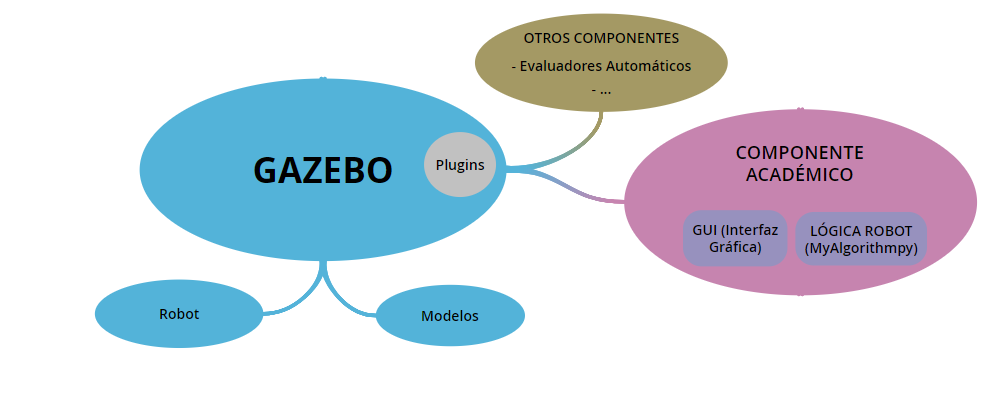
\includegraphics[width=0.9\linewidth]{figures/estructura_jde.png}
		\caption{Estructura de JdeRobot-Academy}
		\label{fig.estructura}
		\end{center}
\end{figure}

En la \textbf{Figura 1.4} se observa que los componentes académicos siguen una arquitectura software que facilita el desarrollo de las prácticas a los alumnos, los cuales únicamente deberán programar su algoritmo, ya sea el pilotaje en función de los datos que proporcionan los sensores o la planificación y el pilotaje con distintos medios. Los componentes académicos cargan el código escrito por el alumno en el fichero plantilla llamado \textit{MyAlgorithm.py} (donde se materializa su resolución), y muestran en la interfaz  gráfica las pruebas o soluciones que realicen los alumnos, distintas trazas de depuración como pueden ser imágenes procesadas, datos láser, imágenes de cámaras integradas,…

Aunque el entorno suele emplear el simulador Gazebo, ha sido desarrollado para que el mismo código implementado en el fichero solución pueda ser ejecutado sobre un robot real. Es por eso que, con el driver adecuado, ese código puede operar un robot físico. El sistema operativo para emplear esta plataforma es Linux, para la cual se ha preparado la infraestructura. Adicionalmente, se ha puesto la vista en crear prácticas abordables desde otras plataformas, utilizado herramientas como la interfaz web de Gazebo, los cuadernillos de Jupyter (ver \textbf{3.6}), tecnologías web de servidor y mediante el empleo de Dockers en vistas a disponer de una versión de la plataforma en MacOS y Windows.
Uno de los ejemplos de prácticas de los que dispone la plataforma es el ejercicio Color Filter que se muestra en la \textbf{Figura 1.5}:

\hspace{0.4\linewidth}
\textit{Color Filter}

\begin{figure}[H]
  \begin{center}
    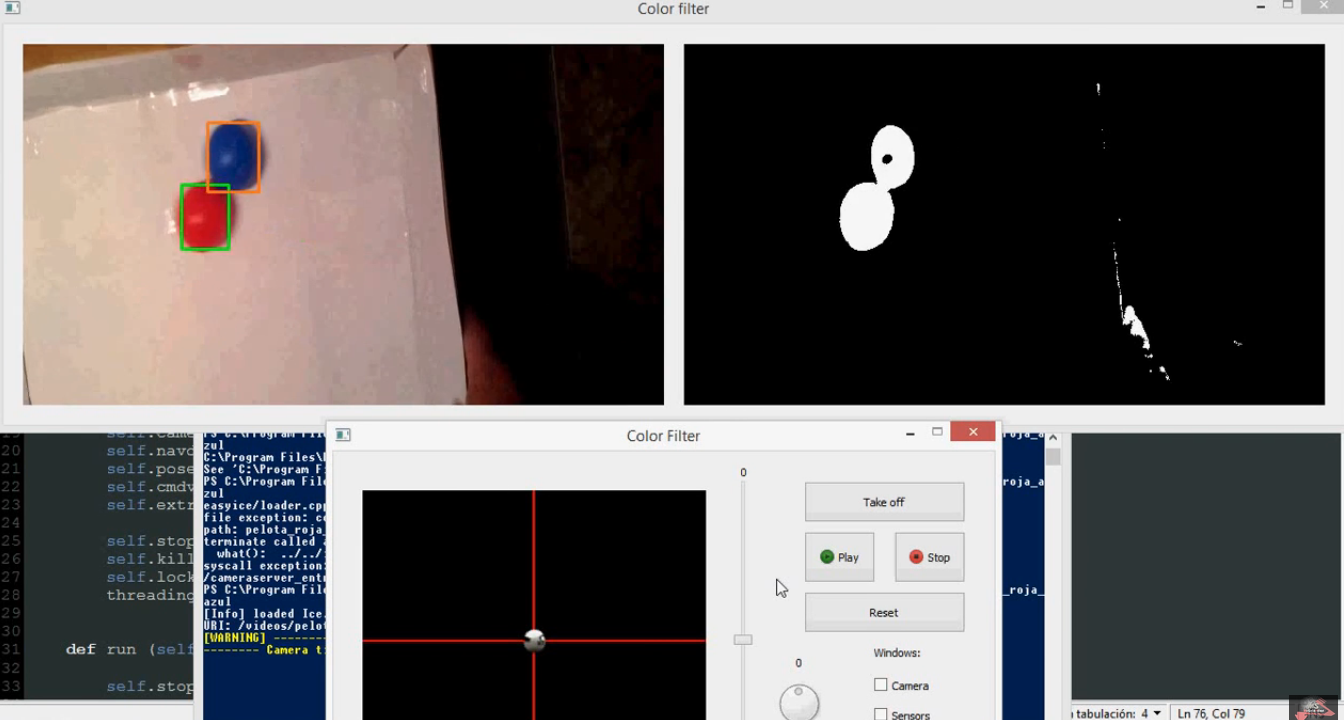
\includegraphics[width=0.95\textwidth]{figures/color_filter.png}
		\caption{Color Filter}
		\label{fig.colorfilter}
		\end{center}
\end{figure}

Donde el alumno puede experimentar con un filtro de color \footnote{\url{https://www.youtube.com/watch?v=tiXagRiqQnY}} aplicado sobre la secuencia de vídeo que proporciona un servidor de imágenes. Su código debe detectar el objeto relevante coloreado (pelotas rojas y azules) utilizando sendos filtros de color, y extraer su posición XY en las imágenes. 

\begin{multicols}{2}

\hspace{0.25\linewidth}
\textit{Bump\&Go}

\begin{figure}[H]
  \begin{center}
    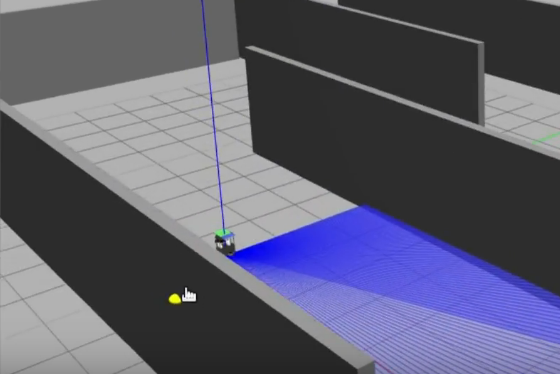
\includegraphics[width=0.98\linewidth, height=5cm]{figures/bumpngo.png}
		\caption{Bump{\&}Go}
		\label{fig.bumpgo}
		\end{center}
\end{figure}

El ejercicio \textit{Bump\&Go} (\textbf{Figura 1.6}) permite implementar una máquina de estados para controlar al robot kobuki en una simulación, un robot diseñado para ser duradero, resistente y rápido, que proporciona al programador acceso a sus motores y a sus sensores láser y de colisión. El alumno debe conseguir que el robot siga el comportamiento típico de chocar y girar, y en última instancia que sea capaz de encontrar la salida del laberinto simulado en el que se encuentra\footnote{\url{http://jderobot.org/store/fperez/uploads/videos/bumpgoo.ogv}}.

\hspace{0.25\linewidth}
\textit{Labyrinth Escape}

\begin{figure}[H]
  \begin{center}
    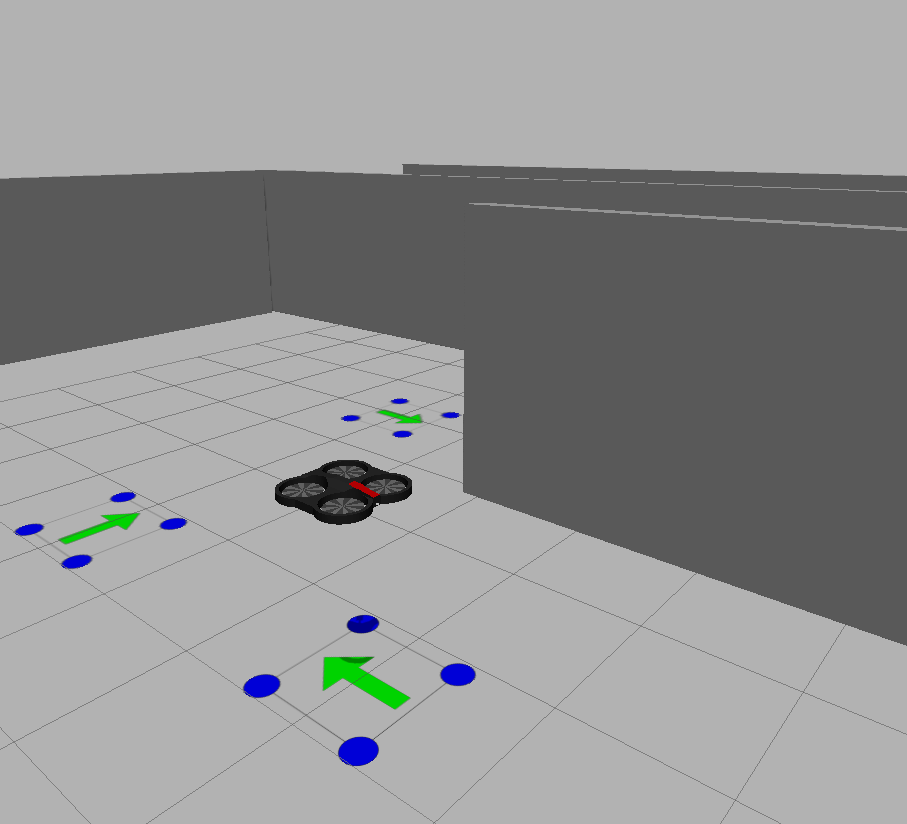
\includegraphics[width=0.98\linewidth, height=5cm]{figures/labyrinth_escape.png}
		\caption{Labyrinth Escape}
		\label{fig.laby}
		\end{center}
\end{figure}

En el ejercicio \textit{Labyrinth Escape} (\textbf{Figura 1.7}), el alumno debe programar la lógica de control de un dron con una cámara incorporada e interfaces de acceso a sus motores para lograr que salga con éxito de un laberinto a través de las imágenes que capta. Para ello, debe hacer uso de las herramientas de procesado y segmentación de imagen para reconocer e interpretar una serie de balizas colocadas a lo largo del escenario que le indican el trazado que debe seguir para encontrar la salida\footnote{\url{https://youtu.be/EdWE5P3uZak}}.

\end{multicols}
\vspace{1cm}
\hspace{0.35\linewidth}
\textit{Obstacle Avoidance}

\begin{figure}[H]
  \begin{center}
    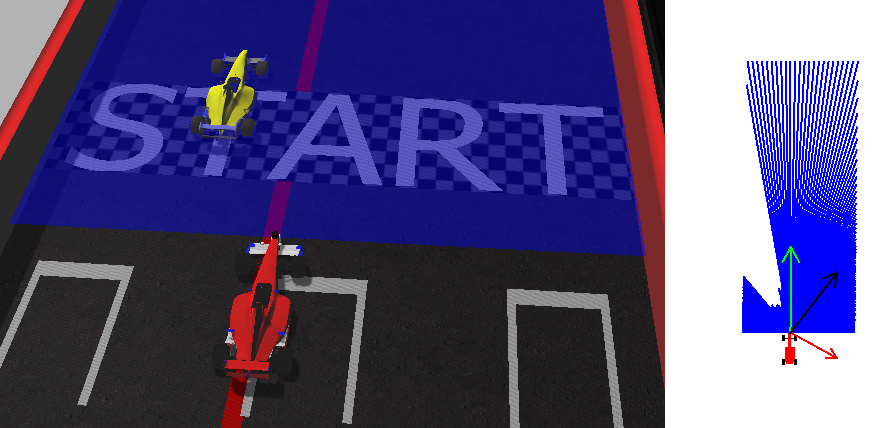
\includegraphics[width=0.95\textwidth, height=5cm]{figures/obstacle_avoidance.png}
		\caption{Obstacle Avoidance}
		\label{fig.obstacleavoidance}
		\end{center}
\end{figure}

En la práctica \textit{Obstacle Avoidance} el estudiante entra en contacto con la tecnología de coches autónomos (en este caso de tipo F1 como se puede ver en la \textbf{Figura 1.8}) equipado con un sensor láser y dos cámaras que ofrecen imágenes desde sus lados izquierdo y derecho. El alumno tendrá que hacer un uso inteligente de la información que el robot pone a su disposición en la simulación para construir una lógica de control y navegación local VFF, el cual se encargará de seguir la carretera del circuito, tomar correctamente las curvas y esquivar los posibles obstáculos que vayan surgiendo en el camino\footnote{\url{https://youtu.be/gVvnrRDmLkI}}.

\hspace{0.35\linewidth}
\textit{Drone-Cat-Mouse}

\begin{figure}[H]
  \begin{center}
    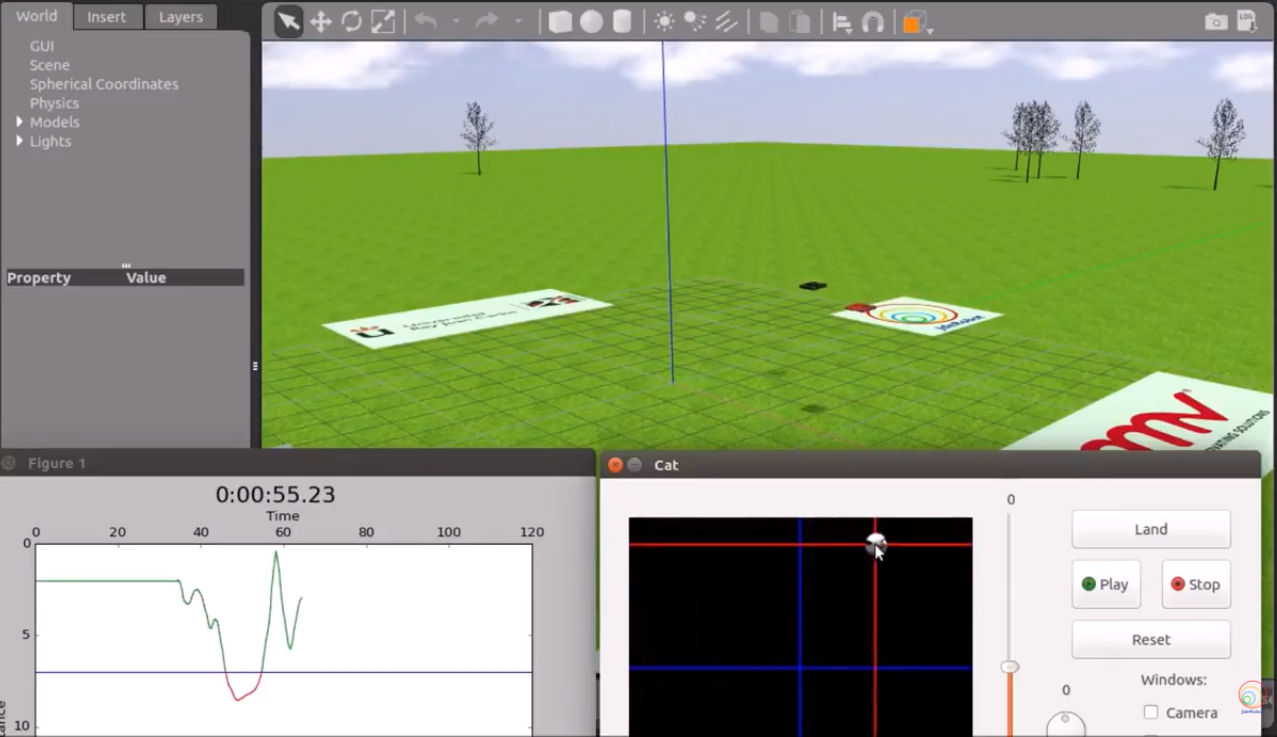
\includegraphics[width=0.95\textwidth, height=7.2cm]{figures/dronecatmouse.png}
		\caption{Drone-Cat-Mouse}
		\label{fig.dronecatmouse}
		\end{center}
\end{figure}

\textit{Drone-Cat-Mouse} es otra de las prácticas del entorno, en la que se ha de programar el dron negro para que persiga al dron rojo (pre-programado con diferentes niveles de dificultad) permaneciendo lo más cerca posible sin colisionar en un entorno simulado al aire libre, emulando el juego del gato y el ratón\footnote{\url{https://www.youtube.com/watch?v=DYD9oPawhWg}}. Esta práctica se  ha empleado en las dos ediciones previas del campeonato \textit{Program-A-Robot}, la primera bajo la organización de la URJC y la segunda en las Jornadas Nacionales de Robótica, que se va a emplear también en la tercera edición dentro de la conferencia internacional IROS\footnote{\url{https://www.iros2018.org/competitions}}.
\vspace{0.6cm}

El objetivo general de este TFG es ampliar las posibilidades de esta plataforma docente, creando nuevas prácticas y mejorando las ya existentes, mejorando su versatilidad. En los próximos capítulos abordaremos todos los elementos necesarios para conseguir este objetivo, empezando por el Capítulo 2, en el que concretaremos los objetivos que se han marcado, así como los requisitos de partida y la metodología empleada. En el Capítulo 3 se expondrá la infraestructura utilizada para llevar a cabo el proyecto. En los Capítulos 4 y 5 se abordarán las prácticas que se han creado. Por último, en el Capítulo 6 se expondrán las conclusiones obtenidas, así como las posibles líneas de mejora que se pueden seguir.

\subsection{Ejercicios recientes}
El contexto inmediato de este trabajo de fin de grado reside en una serie de ejercicios elaborados recientemente también para ampliar las posibilidades de aprendizaje de JdeRobot-Academy. 

Entre ellos, cabe destacar el Trabajo de Fin de Grado de Irene Lope Rodríguez \textit{“Nuevas Prácticas en el Entorno Docente de Robótica JdeRobot-Academy”} , 2018, que se centró en enriquecer la plataforma JdeRobot-Academy con dos nuevas prácticas llamadas “Reconocimiento de la señal stop” o \textit{“car junction”} y “Aspiradora autónoma con autolocalización” o \textit{“vacuum slam”}, la primera de las cuales perseguía que un coche autónomo fuese capaz de reconocer una señal de stop en un cruce vial a través de procesamiento de imágenes provenientes de tres cámaras a bordo del robot, desempeñando el comportamiento habitual ante esta señal de detener el avance, examinar las vías perpendiculares para reconocer posibles coches circulando por ellas y, en caso de que las vías estén libres, girar a la derecha o izquierda para ocupar el carril correspondiente del sentido que se quiera seguir. La segunda de las prácticas que componían este trabajo tenía como objetivo reproducir el comportamiento de limpieza de un robot aspiradora de mercado, eliminado la suciedad en la mayor extensión posible del entorno en que se encuentra, el cual conoce a través de un mapa y un sensor de posición que le ubica en todo momento en la habitación simulada.

También hay que mencionar el Trabajo de Fin de Grado de Vanessa Fernández Martínez \textit{“Nuevas Prácticas en el Entorno Docente de Robótica JdeRobot-Academy”}, 2018, en el que se añadió dos nuevas prácticas al set de ejercicios de JdeRobot-Academy bajo los nombres de “Aspiradora autónoma” o \textit{“vacuum cleaner”} y “Aparcamiento automático” o \textit{“autopark”}, además de mejorarse la práctica ya existente \textit{“TeleTaxi”} con modelos mejorados, un mejor desempeño del algoritmo GPP de navegación global e incluso la inclusión de un evaluador automático capaz de medir el desempeño del algoritmo en función de distintos parámetros para proporcionar al alumno una nota final. En cuanto a los ejercicios creados, \textit{vacuum cleaner} se centró en un algoritmo de navegación sin localización basado en la serie 500 de aspiradoras \textit{Roomba} de iRobot, a través del cual debe recoger la suciedad de la mayor superficie posible de una casa. Por su parte, \textit{autopark} tiene como objetivo implementar un algoritmo basado en estados que permita a un coche autónomo realizar una maniobra de aparcamiento, reconociendo los huecos libres, evitando chocar y respetando los espacios de seguridad a través de los datos sensoriales del robot.

Continuando en esta línea de trabajo, el presente TFG se apoya en la filosofía de estos dos trabajos precedentes para aportar a JdeRobot-Academy dos prácticas que involucren elementos hasta ahora no presentes en las demás: una empleando hardware real y otra haciendo uso de \textit{drivers} de ROS directos.